%!TEX TS-program = xelatex
%!TEX encoding = UTF-8 Unicode

\documentclass[11pt,tikz,border=1]{standalone}
\usetikzlibrary{calc,positioning}

\begin{document}
  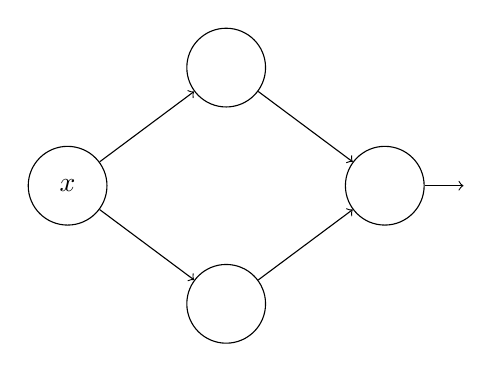
\begin{tikzpicture}[
    neuron/.style={circle,draw,inner sep=0pt,minimum size=10mm}
    ]
    
    \node (l0) [neuron] {$x$};
    \node (m0) [neuron,right=of l0,yshift=-1.5cm] {};
    \node (m1) [neuron,right=of l0,yshift=1.5cm] {};
    \node (r0) [neuron,right=of m0,yshift=1.5cm] {};
    
    \draw[->] (r0) -- ++(1,0);

    \draw[->] (l0) to (m0);
    \draw[->] (l0) to (m1);
    \draw[->] (m0) to (r0);
    \draw[->] (m1) to (r0);

  \end{tikzpicture} 
\end{document}
